


\section{Results}



\subsection{Previous Results}

As mentioned previously, this project is a continuation of a project done over the previous year in
which we developed a method to use pulsar timing data to constrain our models. The final results of
that project were a set of models that accurately reproduce all observables and fully incorporated
the pulsar data. Figure \ref{fig:nobin_obs_panel} shows the model fits to most of the observables
while Figure \ref{fig:nobin_mass_fun} shows the fit to the stellar mass function data. In both
cases, the models satisfyingly reproduce all observables. The median and $1\sigma$ intervals of the
best fit parameters are listed in Table \ref{tab:parameters_nobin}.

One of the most interesting results of the previous project was the models' ability to constrain the
black hole content within 47\,Tuc. Figure \ref{fig:prev_nobin_BH_dists} shows the distribution of
mass in black hole mass and number of black holes in our set of best fit models, which come out to
$240^{+245}_{-146} \mathrm{M}_\odot$ and $41^{+27}_{-22}$ respectively. Both the total mass and
number are quite well contained especially in comparison to the previous constraints in the
literature \citep[see e.g.][]{Henault-Brunet2020,Weatherford2019}.




\begin{table}
	\centering
	\caption{Best fit parameters with $1\sigma$ intervals.}
	\begin{tabular}{l l}

		\hline
		Parameter                 & Value                  \\
		\hline
		$\Phi_0$                  & $6.62^{+0.11}_{-0.11}$ \\
		$M/10^6 \mathrm{M}_\odot$ & $0.88^{+0.01}_{-0.01}$ \\
		$r_h / pc$                & $6.82^{+0.08}_{-0.07}$ \\
		$\log{r_a / pc}$          & $1.33^{+0.04}_{-0.04}$ \\
		$g$                       & $1.03^{+0.08}_{-0.08}$ \\
		$\delta$                  & $0.37^{+0.02}_{-0.01}$ \\
		$s^2$                     & $0.01^{+0.03}_{-0.01}$ \\
		$F$                       & $3.49^{+0.25}_{-0.22}$ \\
		$\alpha_1$                & $0.47^{+0.06}_{-0.05}$ \\
		$\alpha_2$                & $1.18^{+0.06}_{-0.07}$ \\
		$\alpha_3$                & $2.15^{+0.04}_{-0.04}$ \\
		$BH_{ret} (\%)$           & $0.13^{+0.13}_{-0.08}$ \\
		$d$                       & $4.42^{+0.02}_{-0.02}$ \\
		\hline
	\end{tabular}
	\label{tab:parameters_nobin}
\end{table}

\begin{figure}
	\centering
	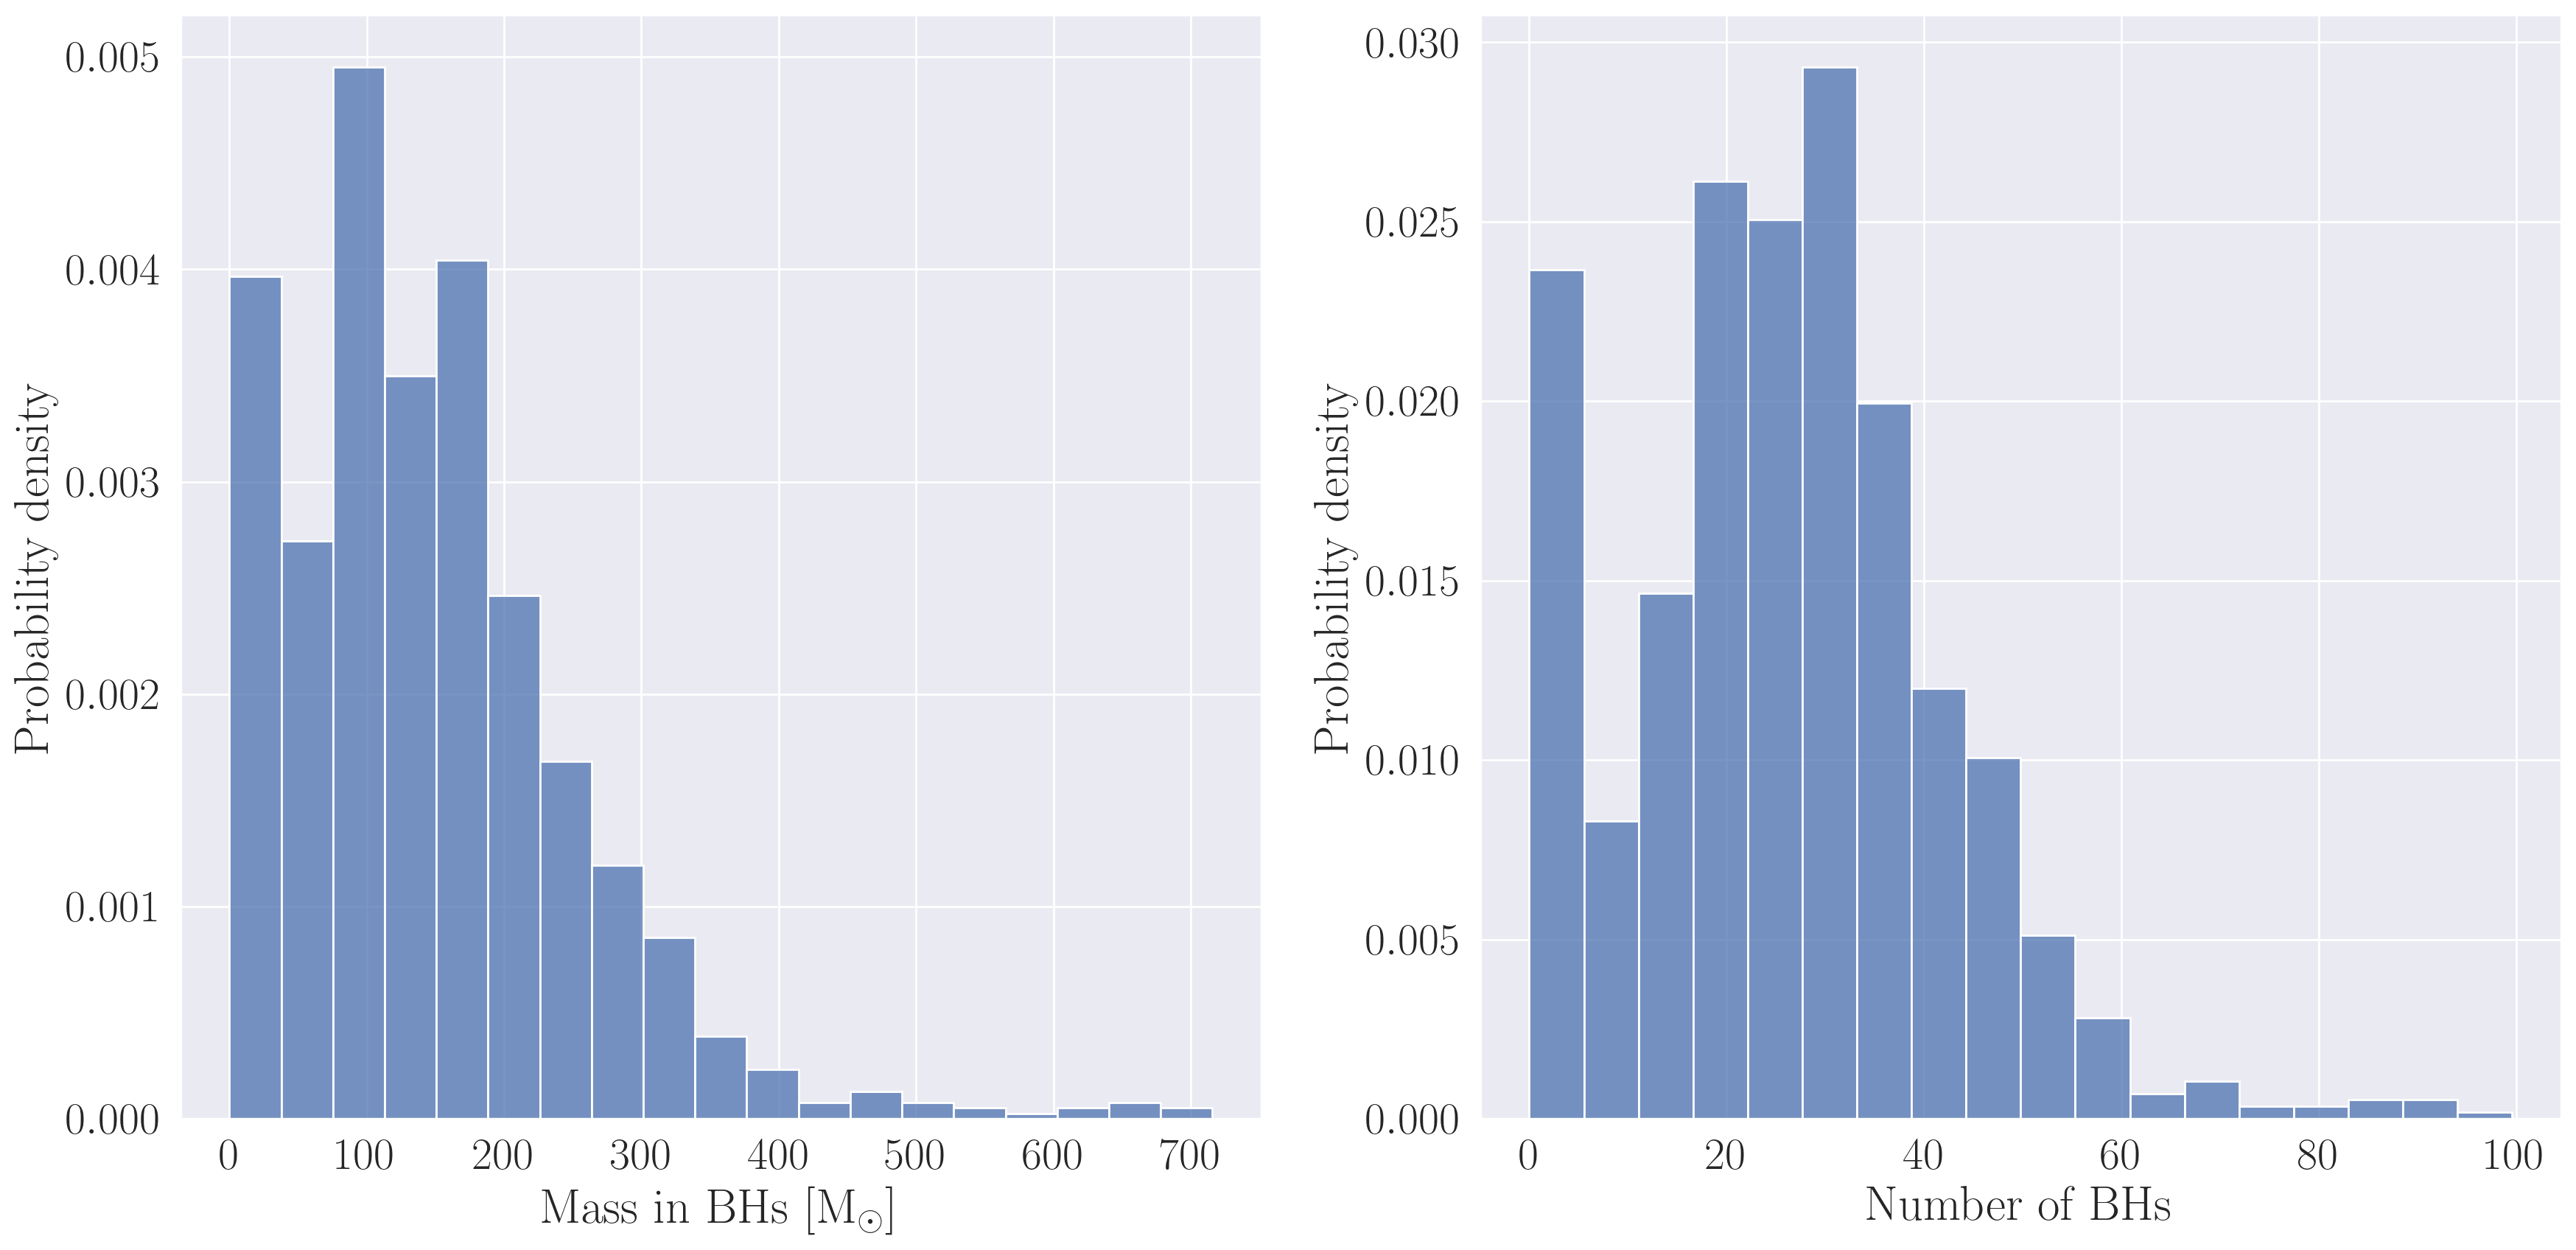
\includegraphics[width=0.8\textwidth]{figures/prev_nobin/BH_dists.png}
	\caption{BH distributions}
	\label{fig:prev_nobin_BH_dists}
\end{figure}


\subsection{Low Binary Fraction}
\ps{Describe the results for the low binary fraction model.}


In the models with a $2\%$ binary fraction, we find a similar ability to reproduce all the
observables, Figure \ref{fig:low_bin_model_obs_panel} and Figure \ref{fig:low_bin_model_mass_fun}
show the model fits compared to the data. Once again the models satisfyingly reproduce all
observables.

The black hole content in these models is also quite well contained, though different from the
models without binaries. Figure \ref{fig:low_bin_model_BH_dists} shows the distribution of mass in
black holes and number of black holes \ps{Which no longer Gaussian, instead use 95, 99 percentile
	limit? Why is this so different from $0\%$ case? This makes me want to rerun the fits for no
	binaries with all the updated data and any other changes.}


$114^{+79}_{-144} \mathrm{M}_\odot$
$22^{+13}_{-19}$ Number


The best-fit parameters and their $1\sigma$ intervals are listed in Table \ref{tab:parameters_lowbin}.


\begin{table}
	\centering
	\caption{Best fit parameters with $1\sigma$ intervals.}
	\begin{tabular}{l l}

		\hline
		Parameter                 & Value                  \\
		\hline
		$\Phi_0$                  & $6.28^{+0.10}_{-0.10}$ \\
		$M/10^6 \mathrm{M}_\odot$ & $0.89^{+0.01}_{-0.01}$ \\
		$r_h / pc$                & $6.74^{+0.06}_{-0.06}$ \\
		$\log{r_a / pc}$          & $1.50^{+0.06}_{-0.05}$ \\
		$g$                       & $1.36^{+0.06}_{-0.06}$ \\
		$\delta$                  & $0.43^{+0.02}_{-0.02}$ \\
		$s^2$                     & $0.01^{+0.01}_{-0.00}$ \\
		$F$                       & $3.24^{+0.13}_{-0.12}$ \\
		$\alpha_1$                & $0.37^{+0.02}_{-0.02}$ \\
		$\alpha_2$                & $1.47^{+0.05}_{-0.05}$ \\
		$\alpha_3$                & $2.18^{+0.04}_{-0.04}$ \\
		$BH_{ret} (\%)$           & $0.08^{+0.09}_{-0.05}$ \\
		$d$                       & $4.42^{+0.02}_{-0.02}$ \\
		\hline
	\end{tabular}
	\label{tab:parameters_lowbin}
\end{table}

\begin{figure}
	\centering
	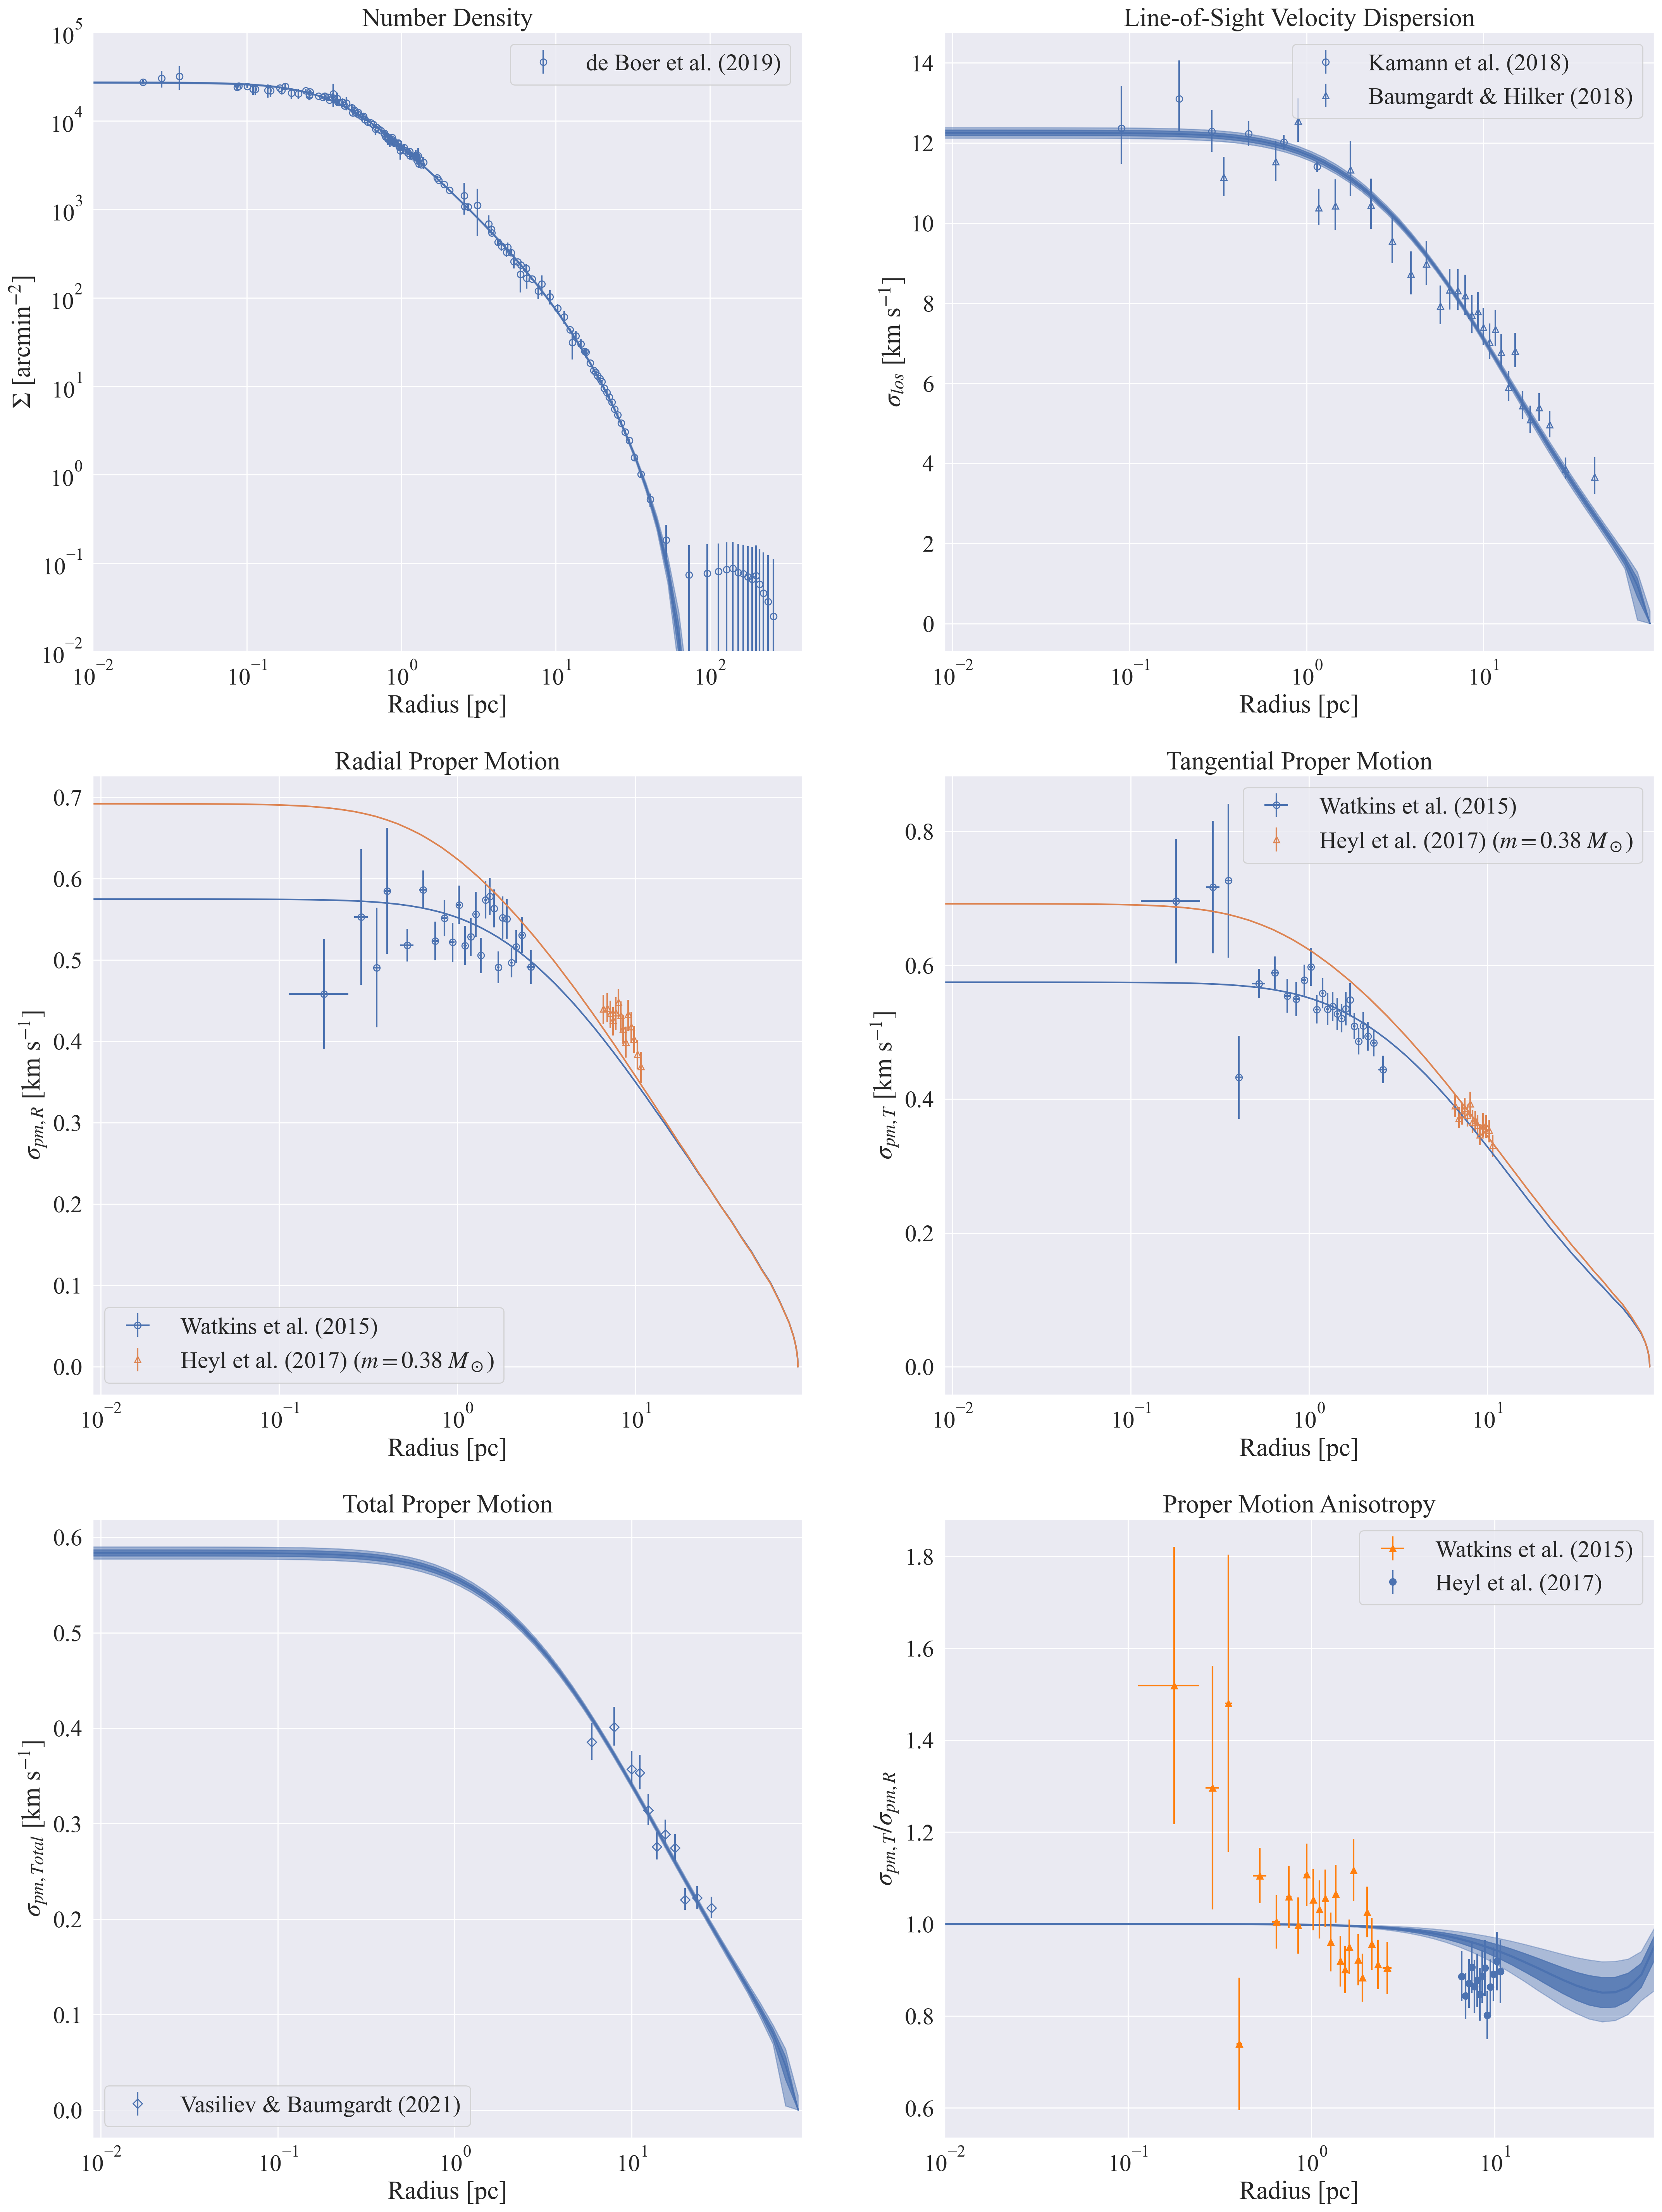
\includegraphics[width=0.9\textwidth]{figures/low_bin_model/obs_panel.png}
	\caption{Observables}
	\label{fig:low_bin_model_obs_panel}
\end{figure}


\begin{figure}
	\centering
	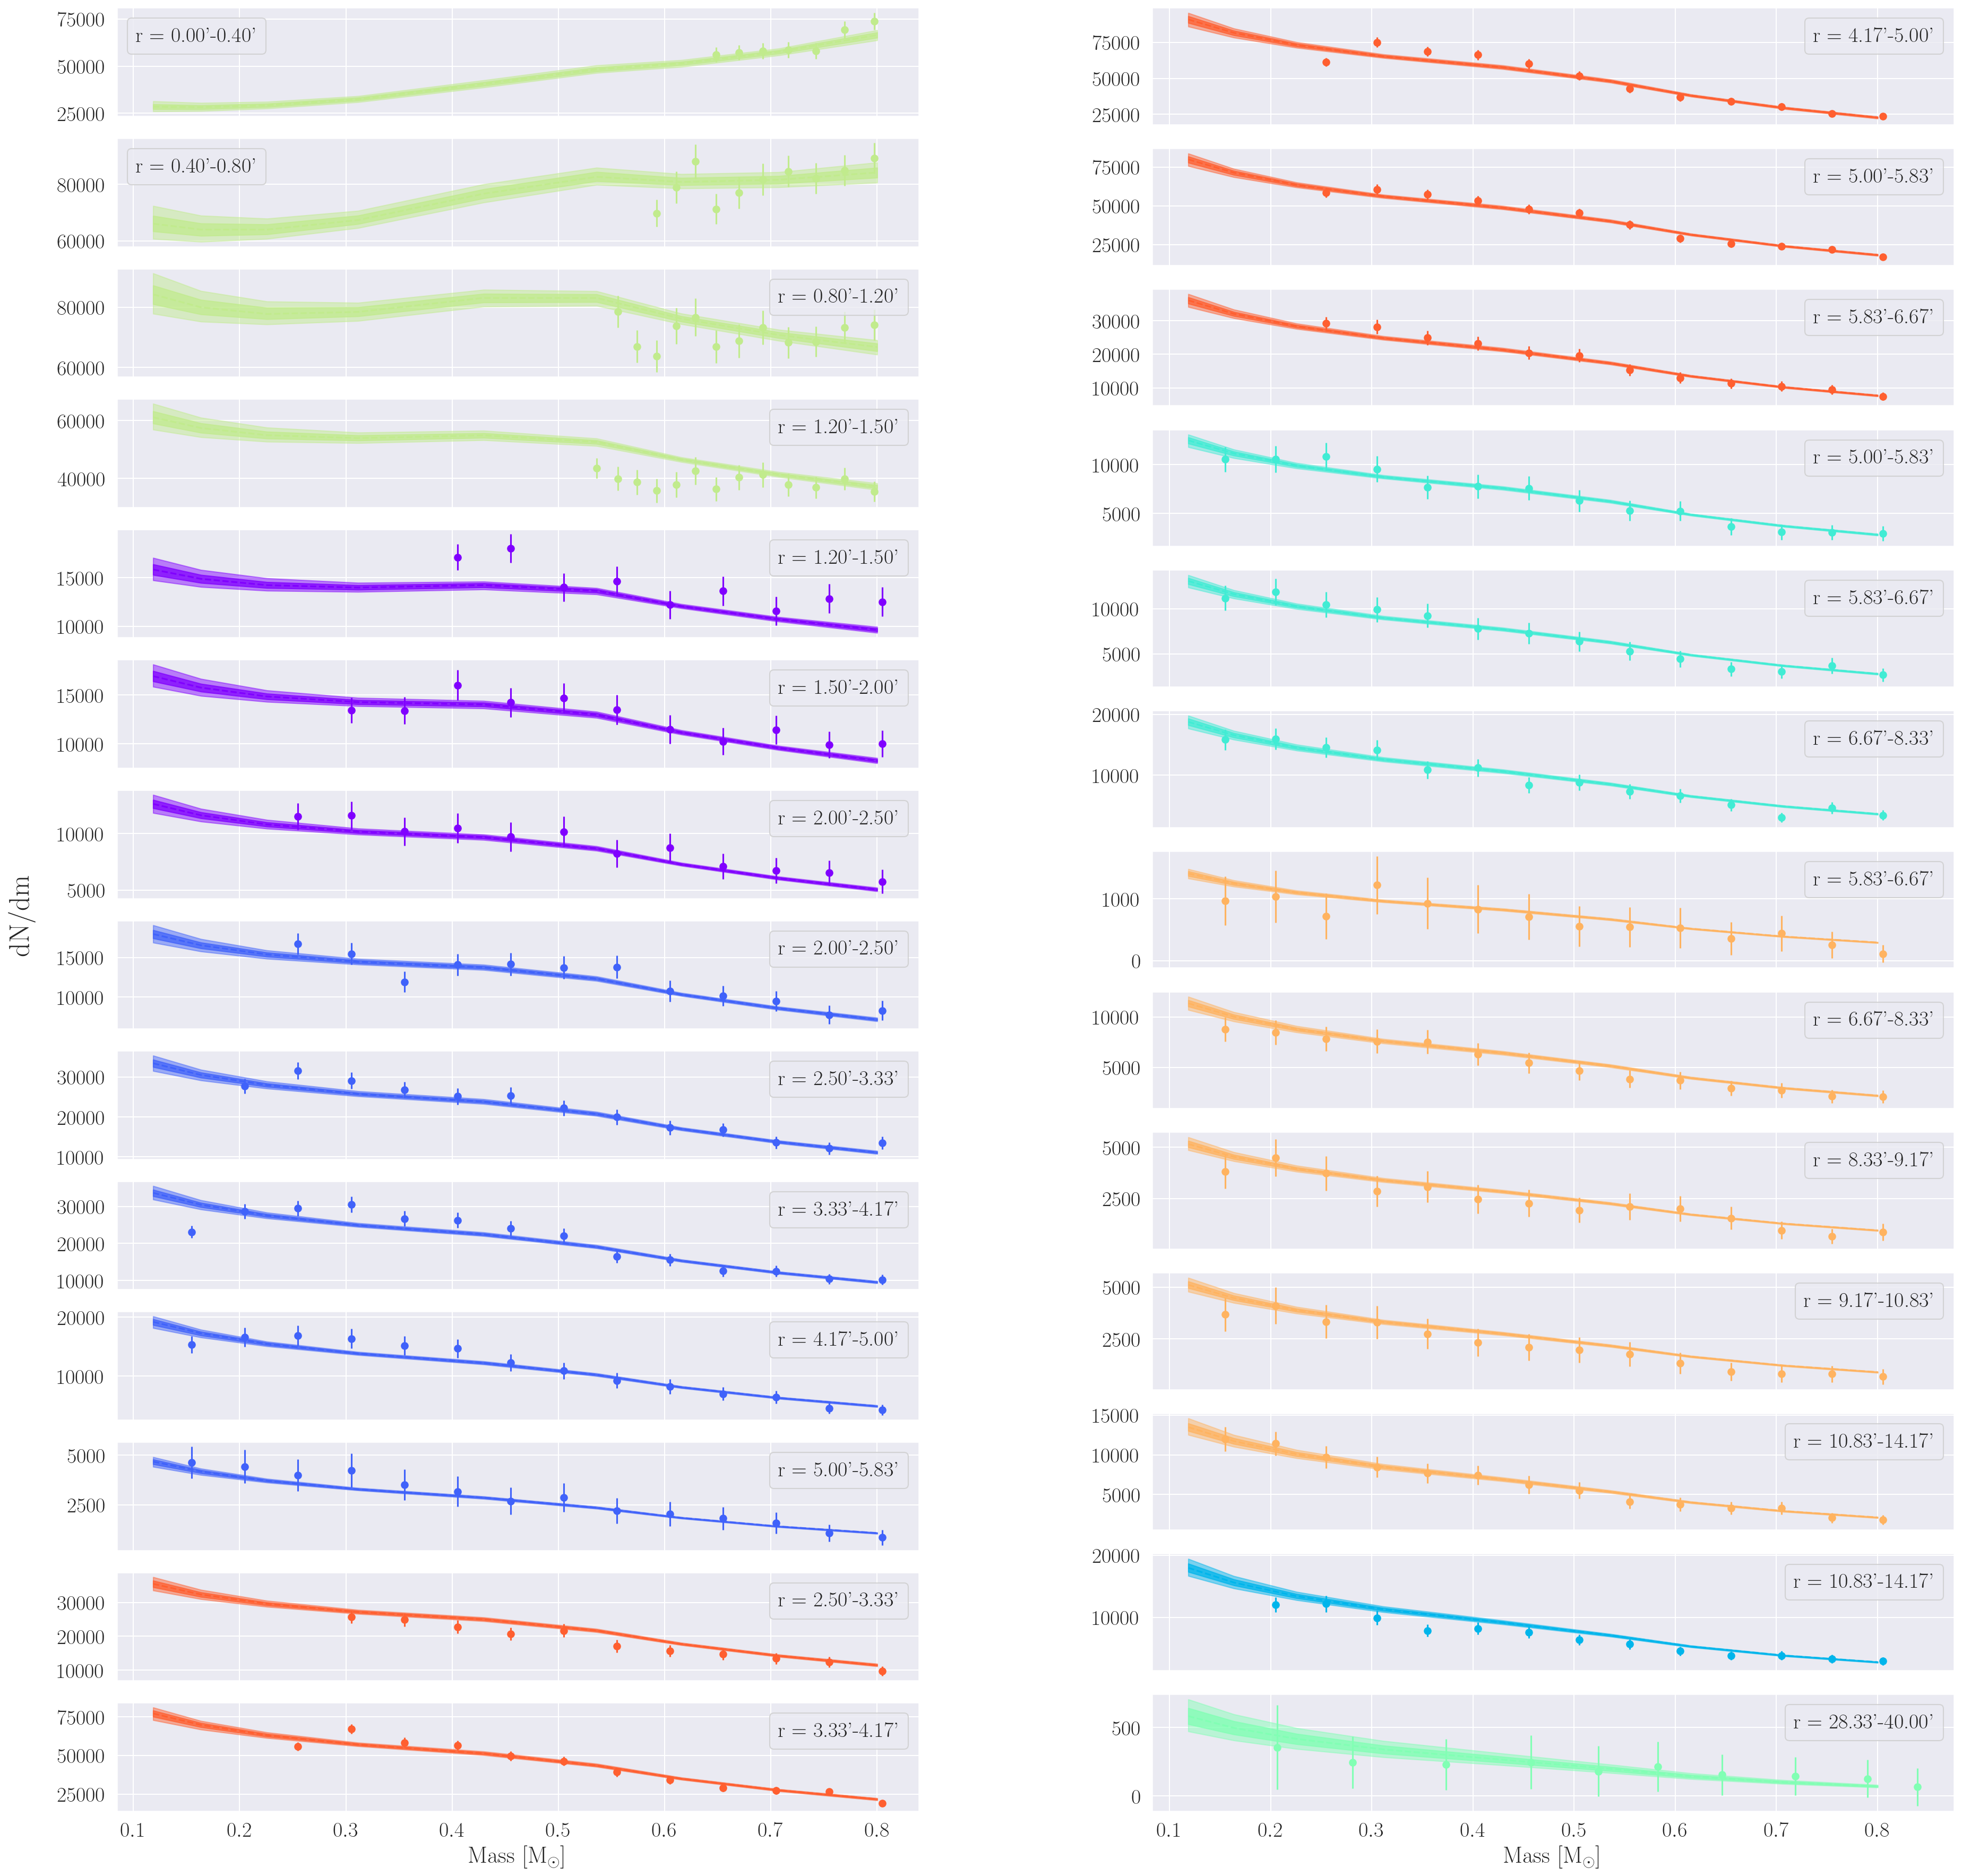
\includegraphics[width=\textwidth]{figures/low_bin_model/mass_fun.png}
	\caption{Mass function}
	\label{fig:low_bin_model_mass_fun}
\end{figure}



\begin{figure}
	\centering
	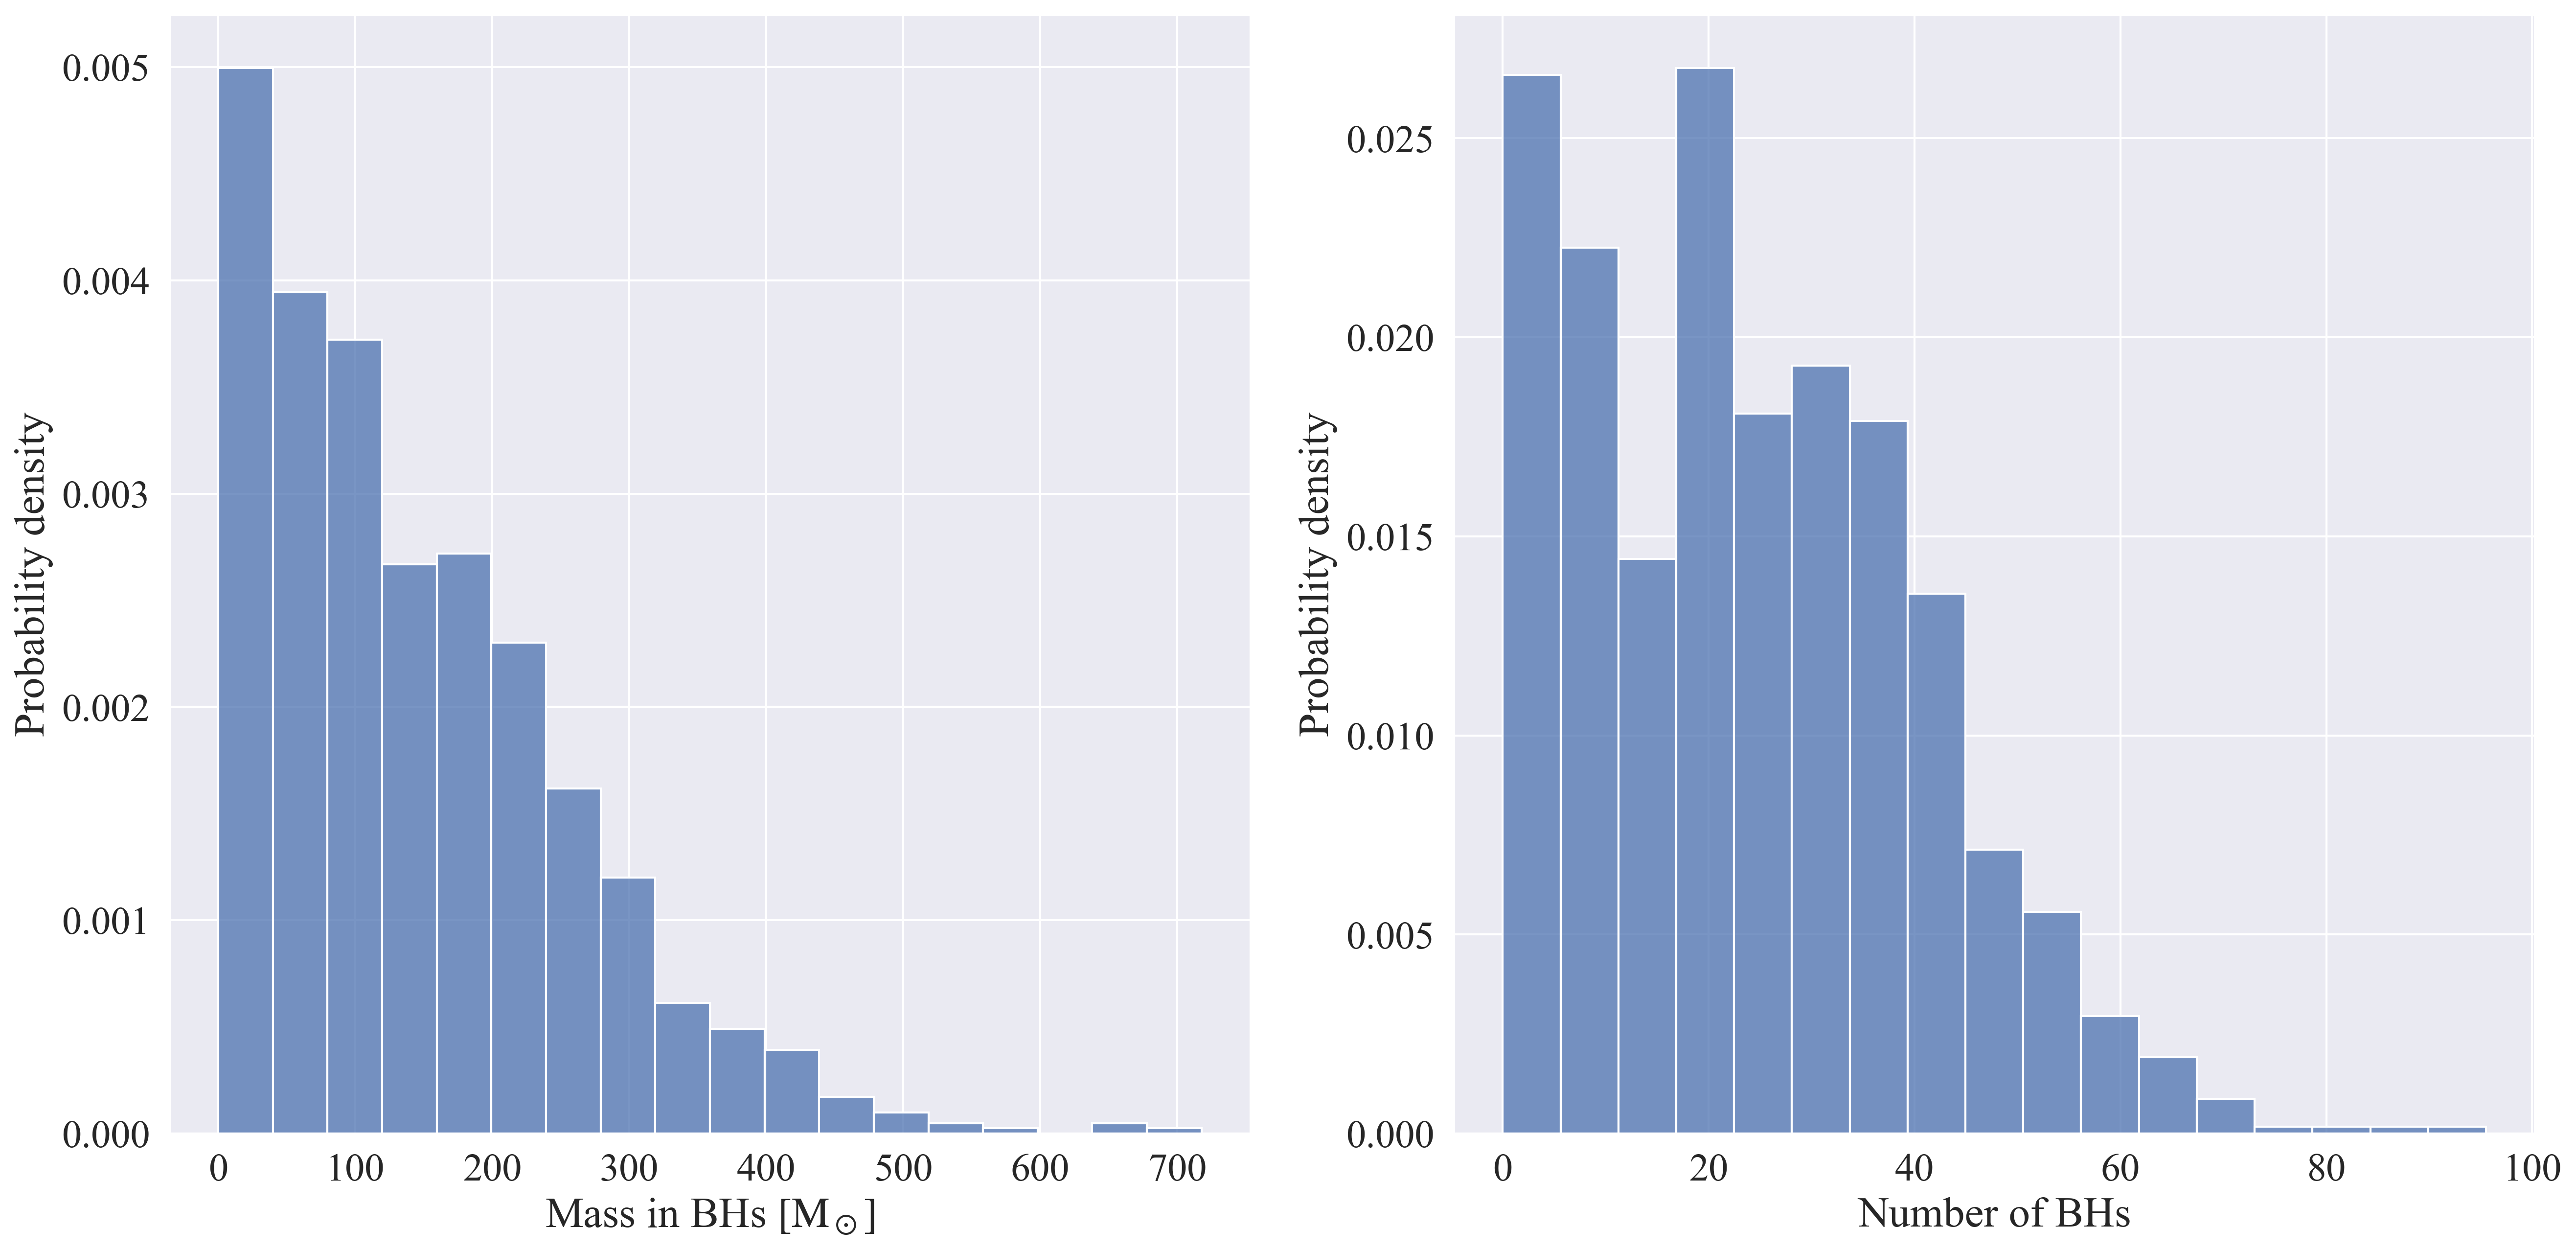
\includegraphics[width=0.8\textwidth]{figures/low_bin_model/BH_dists.png}
	\caption{BH distributions}
	\label{fig:low_bin_model_BH_dists}
\end{figure}


A binary fraction of $2\%$ results in a total mass in binaries of around $15800 \mathrm{M}_\odot$,
Figure \ref{fig:low_bin_model_Bin_mass} shows the distribution of mass in binaries in our set of
best-fitting models.


\begin{figure}
	\centering
	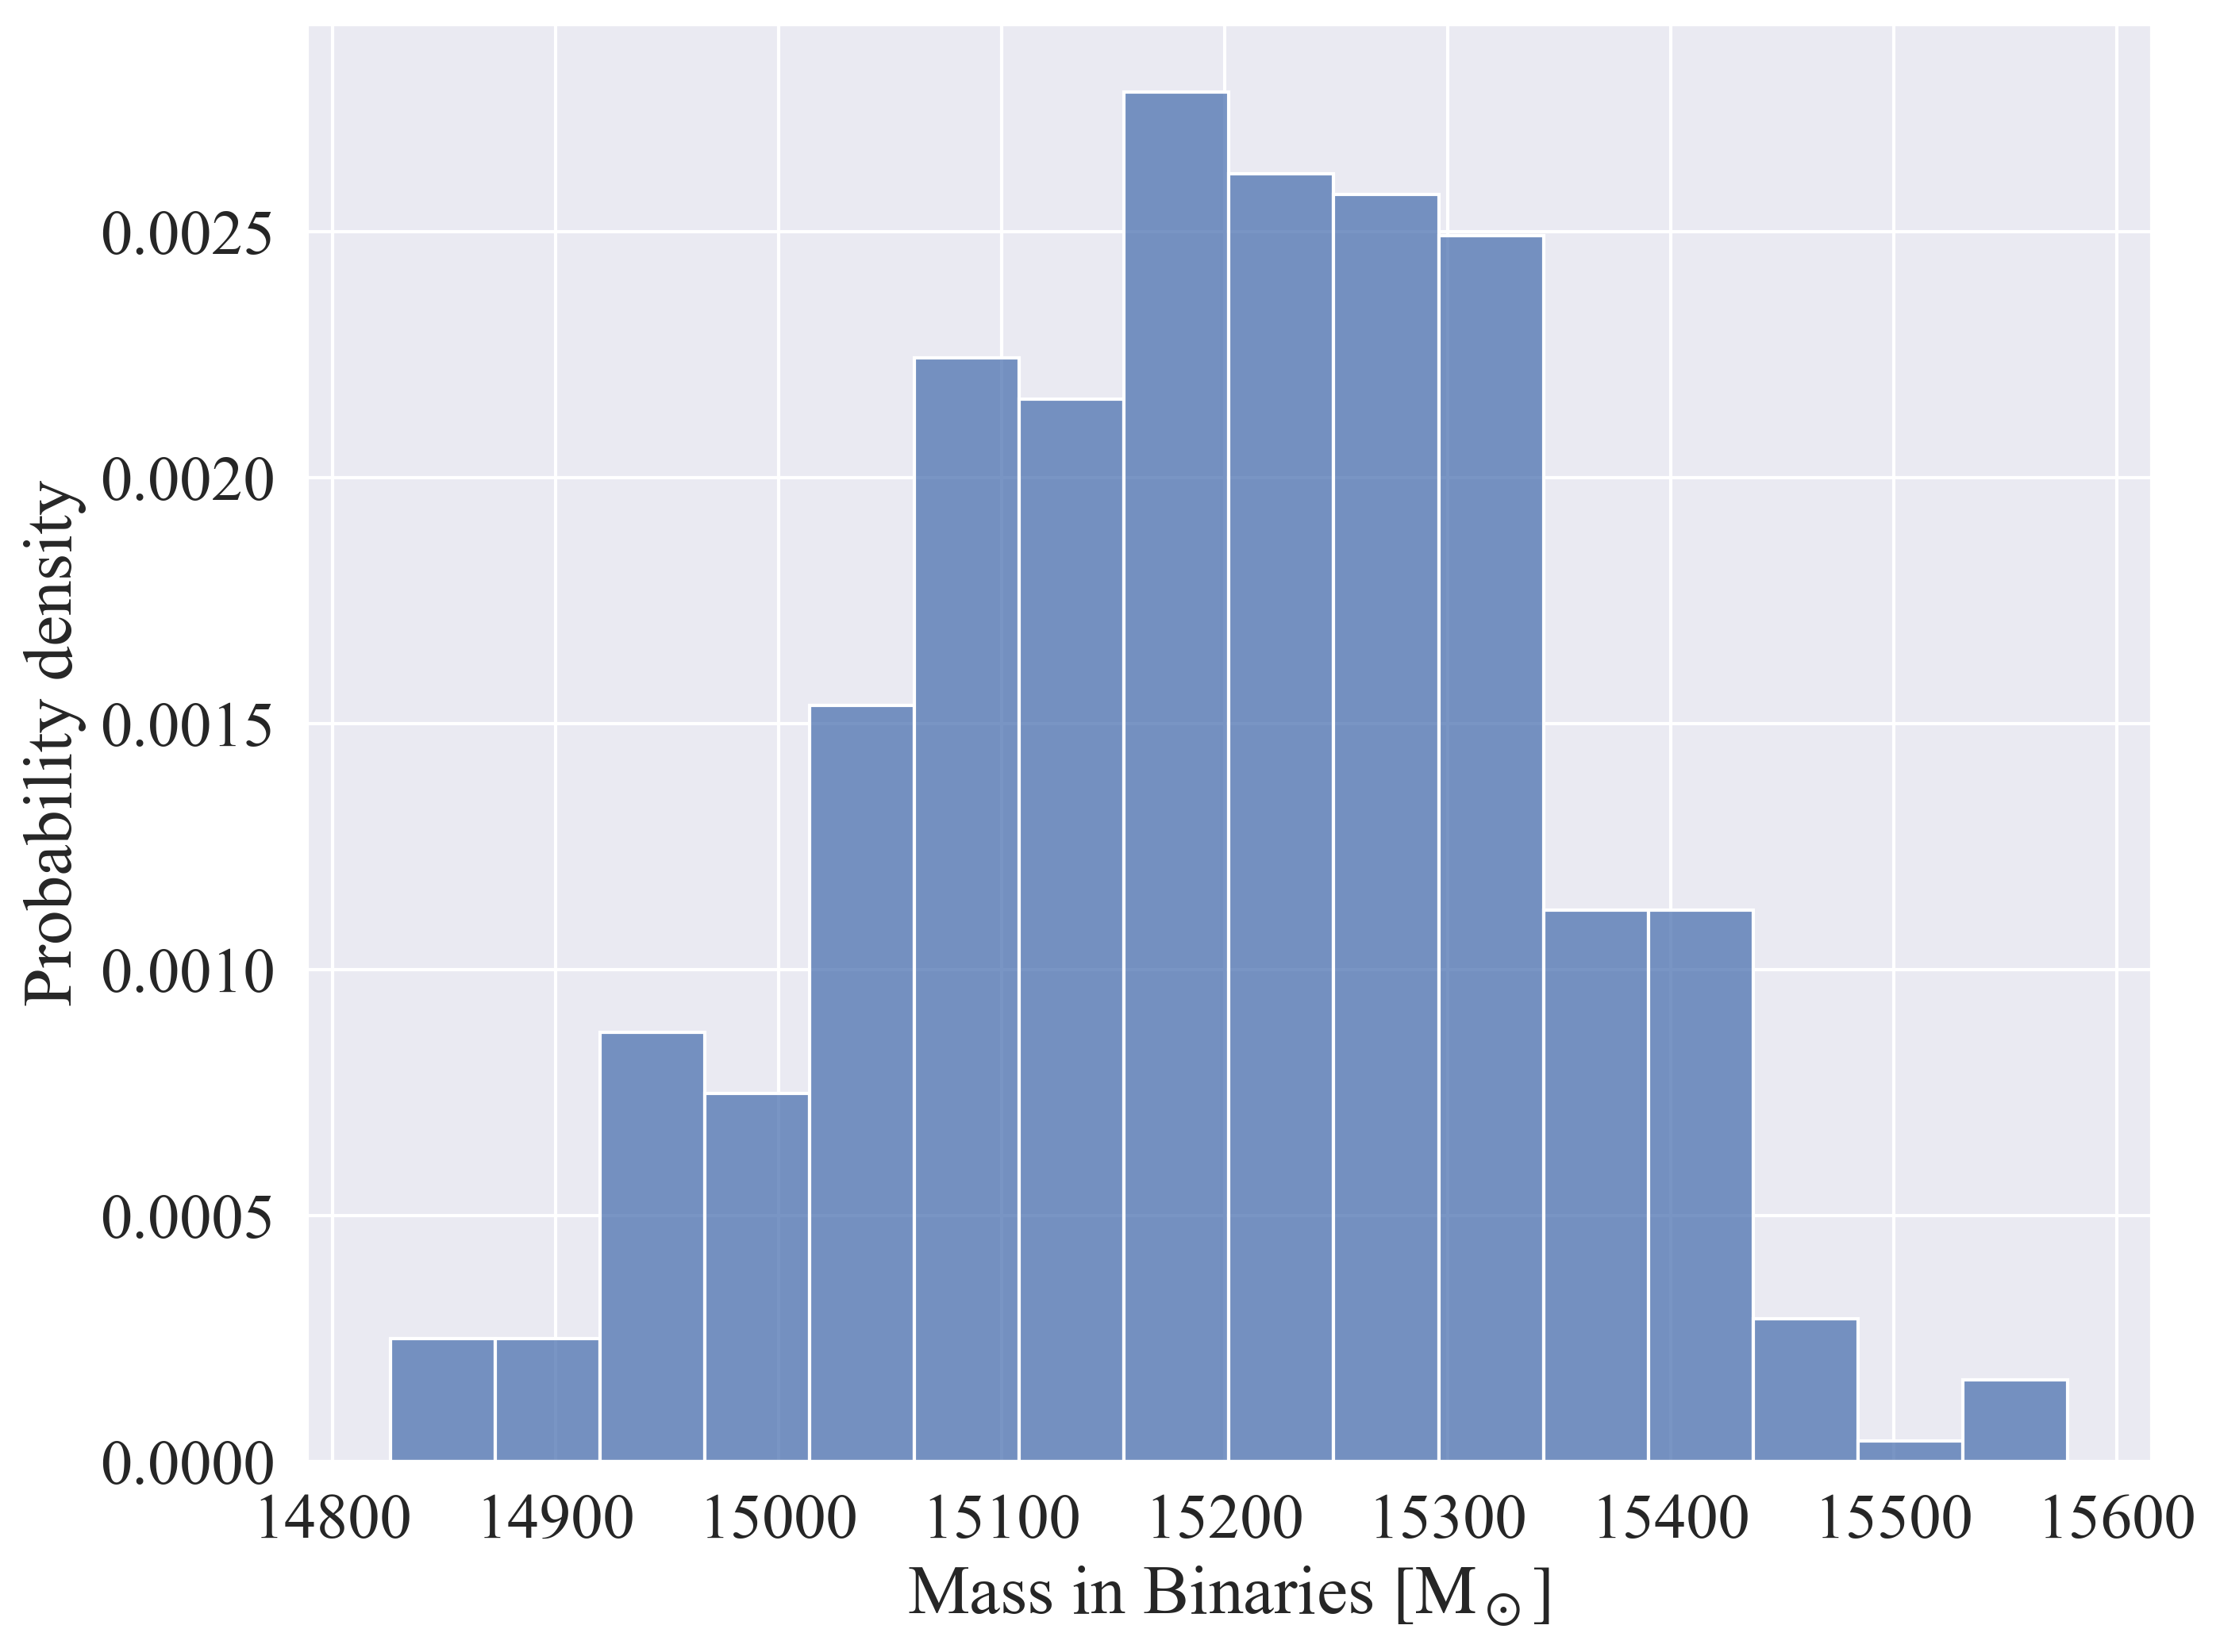
\includegraphics[width=0.8\textwidth]{figures/low_bin_model/binary_mass.png}
	\caption{Mass in Binaries}
	\label{fig:low_bin_model_Bin_mass}
\end{figure}


\subsection{High Binary Fraction}

As is the case for the models with a low binary fraction, the models with a $10\%$ binary
fraction fit the observables very well. Figures \ref{fig:highbin_obs_panel} and
\ref{fig:highbin_mass_fun} show the model fits compared to the data.

\begin{table}
	\centering
	\caption{Best fit parameters with $1\sigma$ intervals.}
	\begin{tabular}{l l}

		\hline
		Parameter                 & Value                  \\
		\hline
		$\Phi_0$                  & $6.36^{+0.09}_{-0.09}$ \\
		$M/10^6 \mathrm{M}_\odot$ & $0.89^{+0.01}_{-0.01}$ \\
		$r_h / pc$                & $6.77^{+0.06}_{-0.06}$ \\
		$\log{r_a / pc}$          & $1.48^{+0.06}_{-0.05}$ \\
		$g$                       & $1.34^{+0.06}_{-0.06}$ \\
		$\delta$                  & $0.41^{+0.01}_{-0.01}$ \\
		$s^2$                     & $0.01^{+0.01}_{-0.00}$ \\
		$F$                       & $3.16^{+0.13}_{-0.12}$ \\
		$\alpha_1$                & $0.45^{+0.02}_{-0.02}$ \\
		$\alpha_2$                & $1.53^{+0.05}_{-0.04}$ \\
		$\alpha_3$                & $2.46^{+0.05}_{-0.05}$ \\
		$BH_{ret} (\%)$           & $0.17^{+0.18}_{-0.12}$ \\
		$d$                       & $4.43^{+0.02}_{-0.02}$ \\
		\hline
	\end{tabular}
	\label{tab:parameters_highbin}
\end{table}


$81 ^{+81}_{-121} \mathrm{M}_\odot$
$12^{+12}_{-13}$

\begin{figure}
	\centering
	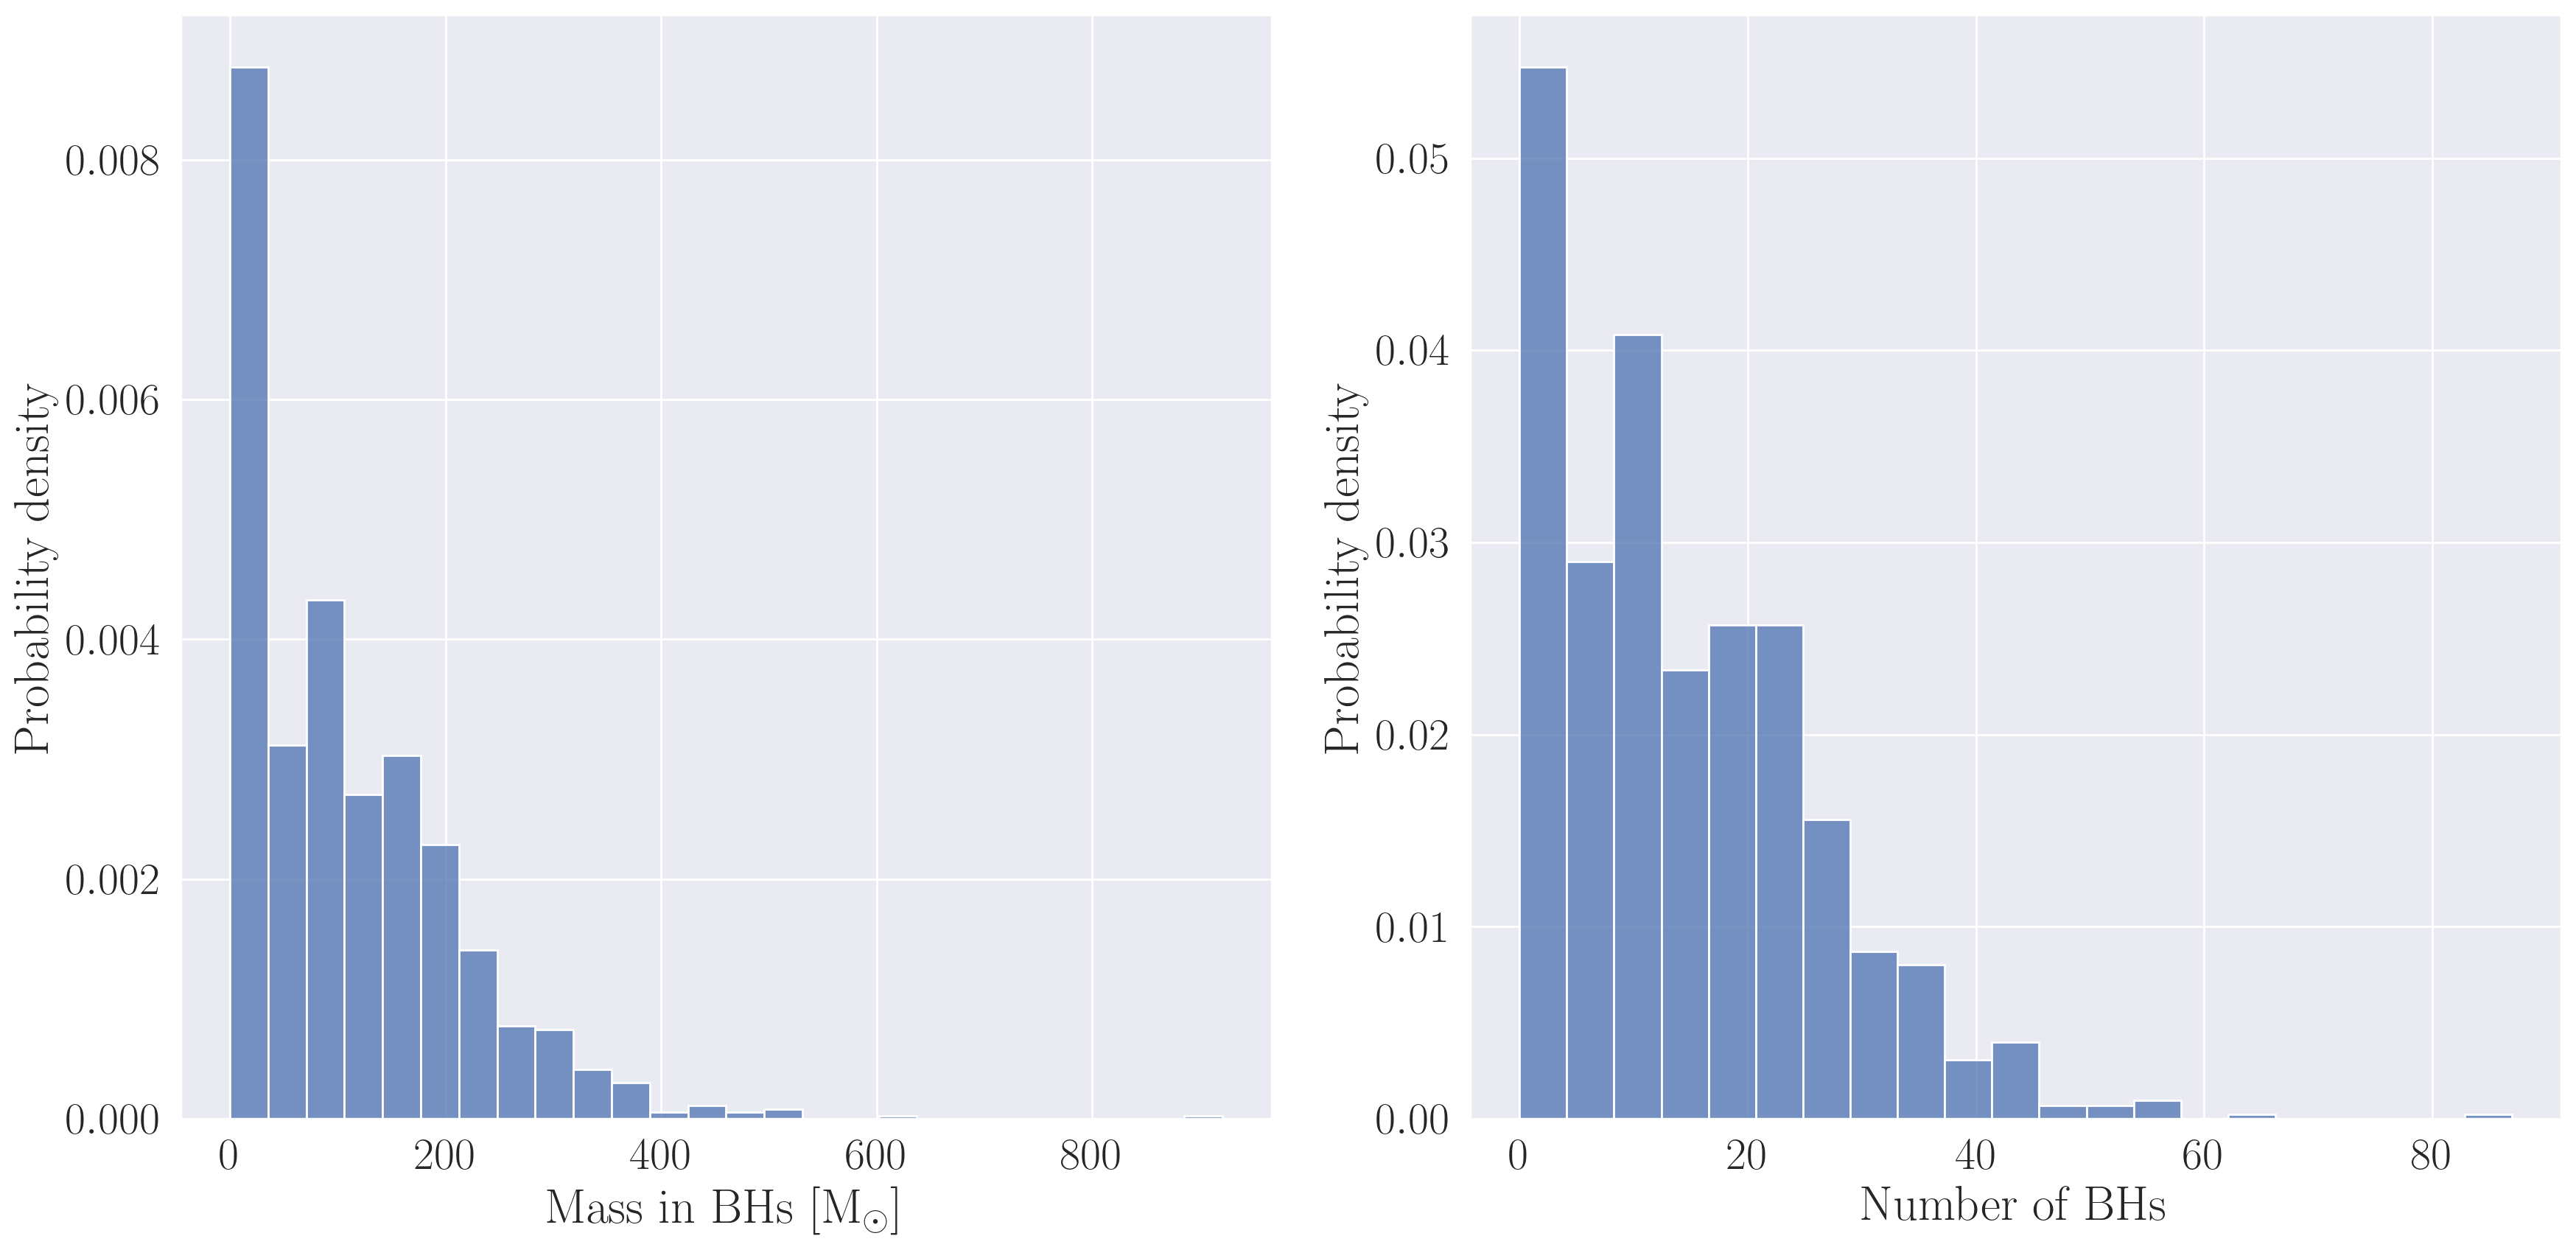
\includegraphics[width=0.8\textwidth]{figures/high_bin_model/BH_dists.png}
	\caption{BH distributions}
	\label{fig:high_bin_model_BH_dists}
\end{figure}


Now around $81000 \mathrm{M}_\odot$ in binaries.

\begin{figure}
	\centering
	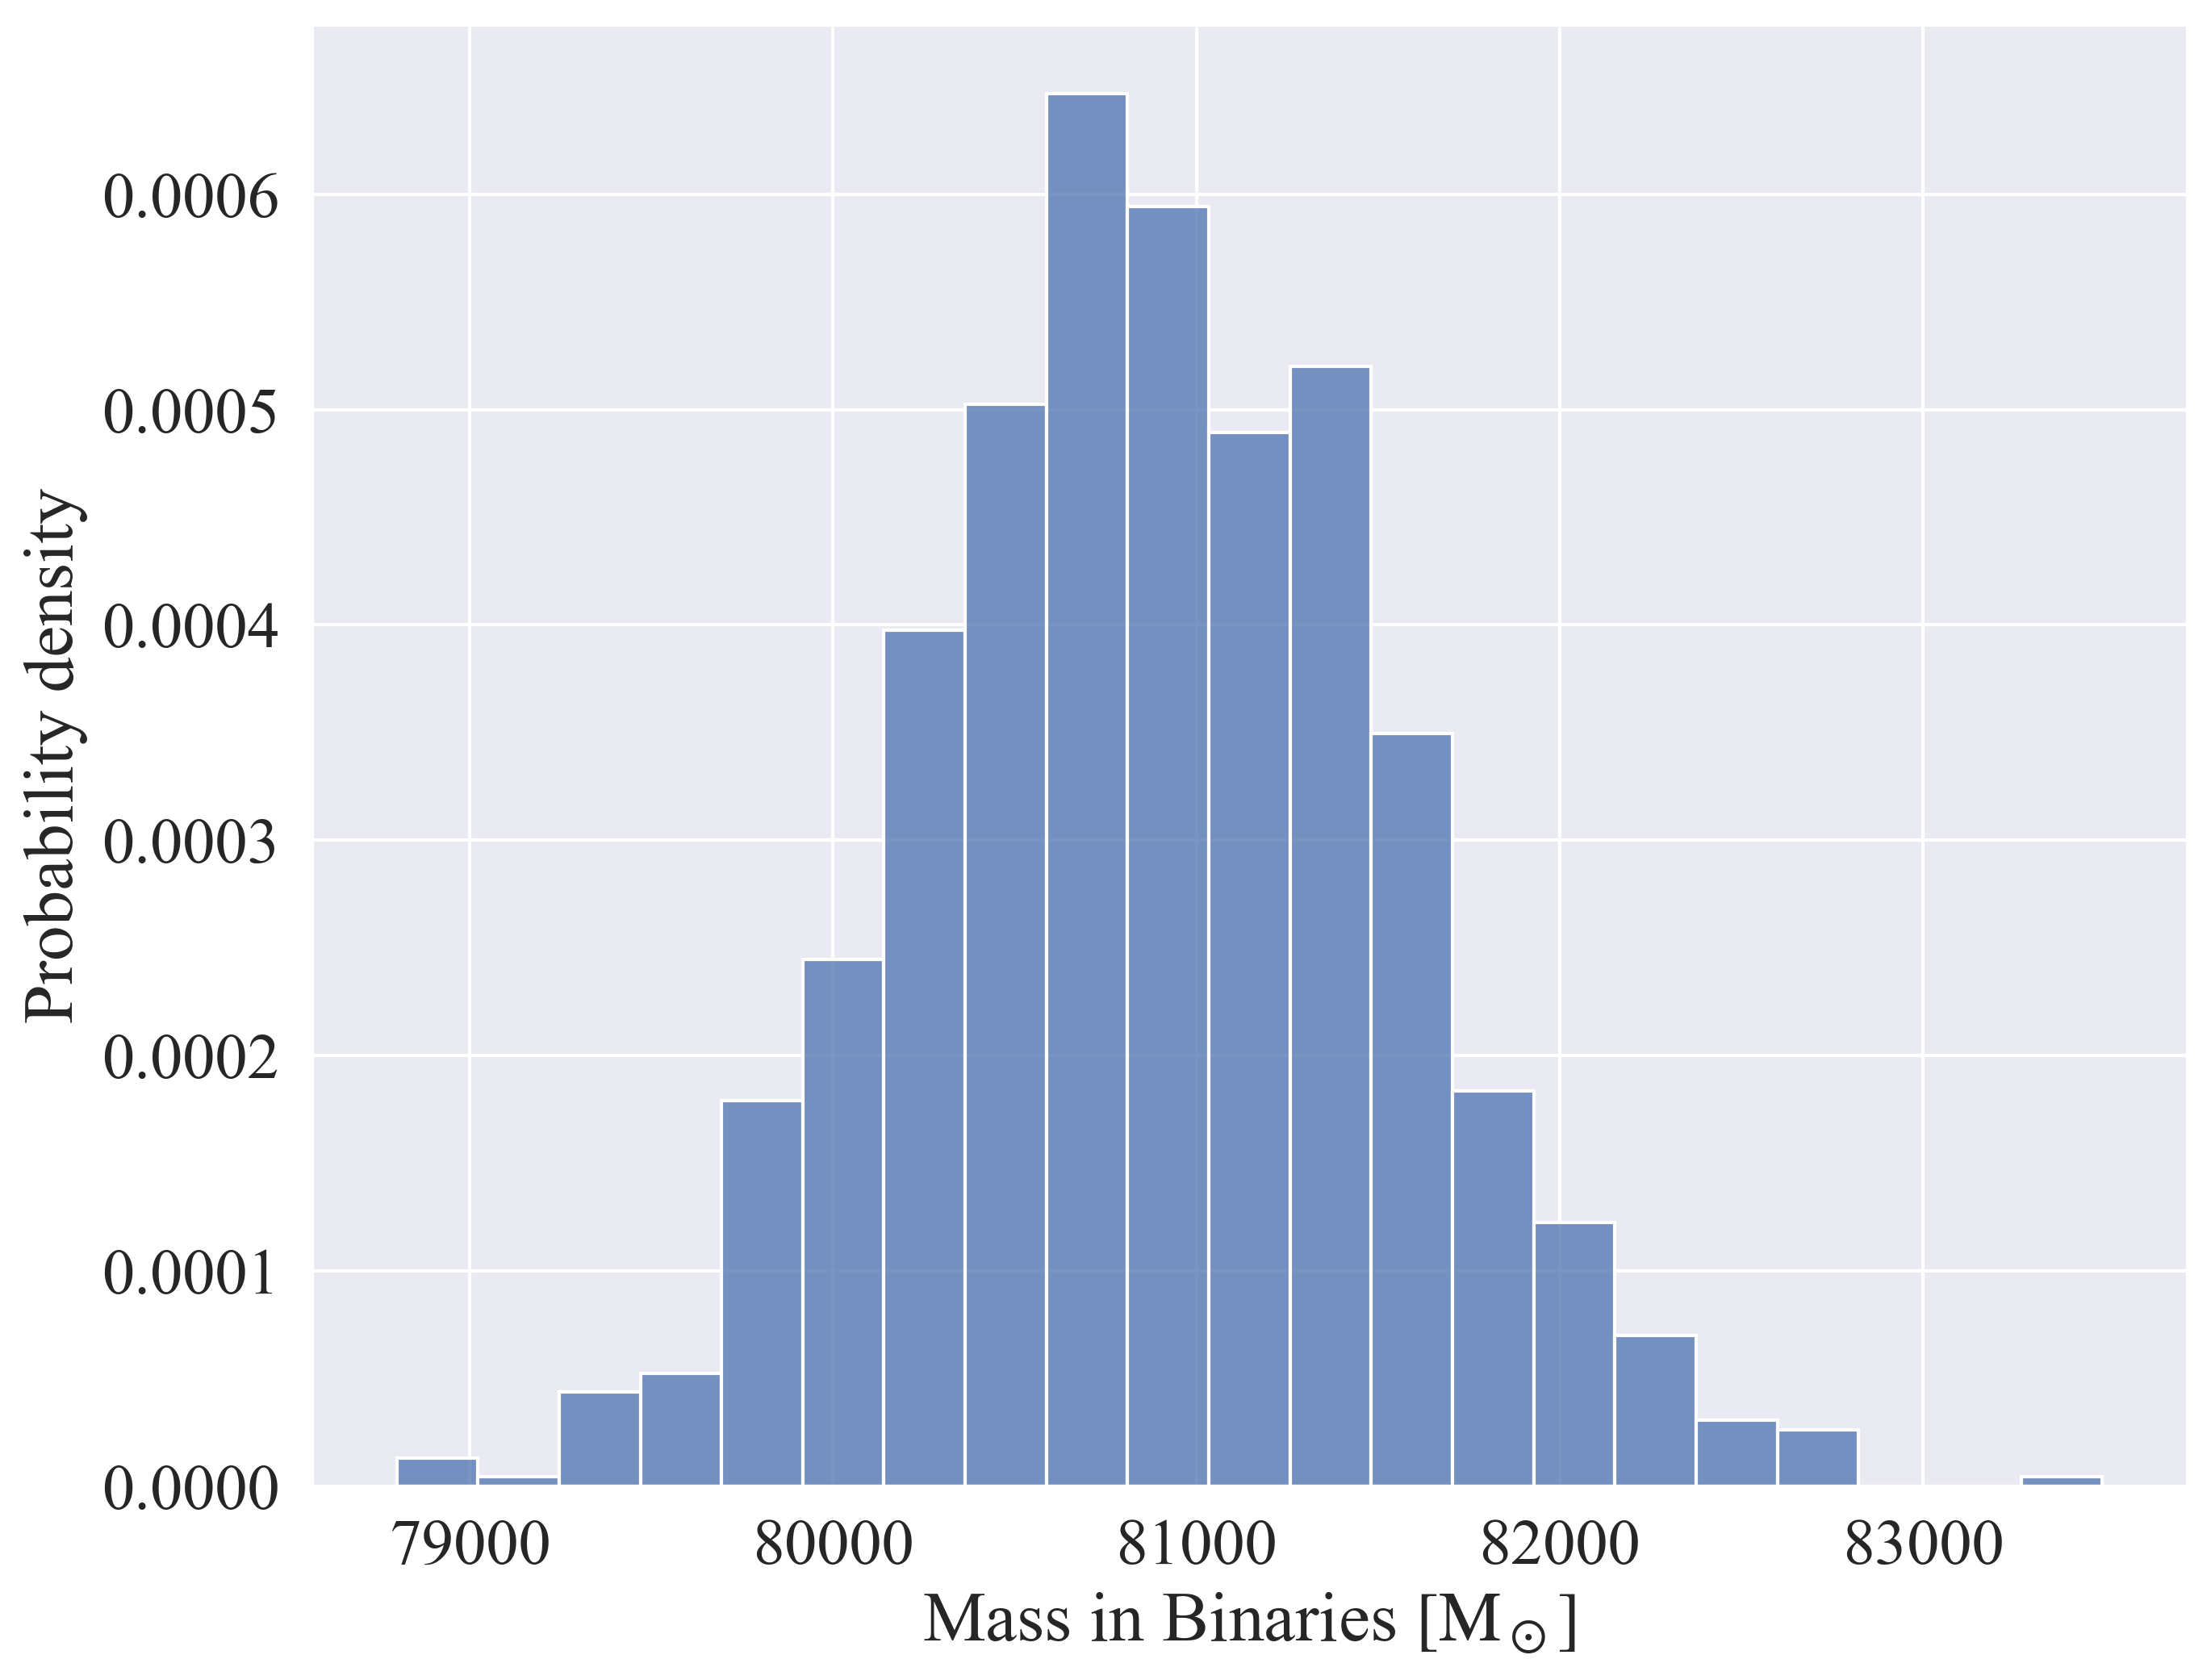
\includegraphics[width=0.8\textwidth]{figures/high_bin_model/binary_mass.png}
	\caption{Binary Mass}
	\label{fig:high_bin_model_Bin_mass}
\end{figure}





\section{Discussion}



In each set of models, all observables are very well reproduced, showing the flexibility of the
\code{LIMEPY} models. Due to this flexibility, it is unlikely that with current observations we
would be able to infer anything about the binary population of a cluster using this technique.
Instead, this method should be used in cases where there are existing estimates of the binary
population within a cluster in order to add a realistic binary component to \code{LIMEPY} models

All three sets of models mostly agrees in terms of the recovered model parameters. In particular,
the total cluster mass is identical in each set of models.

\ps{I'm thinking this might be even more pronounced after we rerun the no binary case}


\subsection{The effects of the binaries}



Table \ref{tab:BH_contents} shows the distribution of BHs for each set of models. We can see a clear
decrease in the black hole content as we add more and more binaries. This effect was also found by
\citet{Mann2019} (see also associated erratum \citealt{Mann2020}) when they modelled the central
kinematic of 47\,Tuc.

% Table comparing bh content in each set of models
\begin{table}

\centering
\caption{Binary fraction in each set of models}
\begin{tabular}{c c c}
	\hline
	Binary Fraction $(\%)$ & Mass in BHs                          & Number of BHs    \\
	\hline
	0                      & $240^{+245}_{-146} \mathrm{M}_\odot$ & $41^{+27}_{-22}$ \\
	2                      & $114^{+79}_{-144} \mathrm{M}_\odot$  & $22^{+13}_{-19}$ \\
	10                     & $81 ^{+81}_{-121} \mathrm{M}_\odot$  & $12^{+12}_{-13}$ \\
	\hline
\end{tabular}
\label{tab:BH_contents}
\end{table}



When we examine the density profiles for the models with a binary fraction of $10\%$ (see Figure
\ref{fig:highbin_model_densities}), we can see that the binary stars are indeed more centrally
concentrated than typical main-sequence stars as predicted and in the central regions, actually
contribute more to mass density than single stars \ps{Is this true? The MS profile includes the
	binaries too (I think), why is it lower?}, while they contribute more than the neutron stars at all
radii.


\begin{figure}
	\centering
	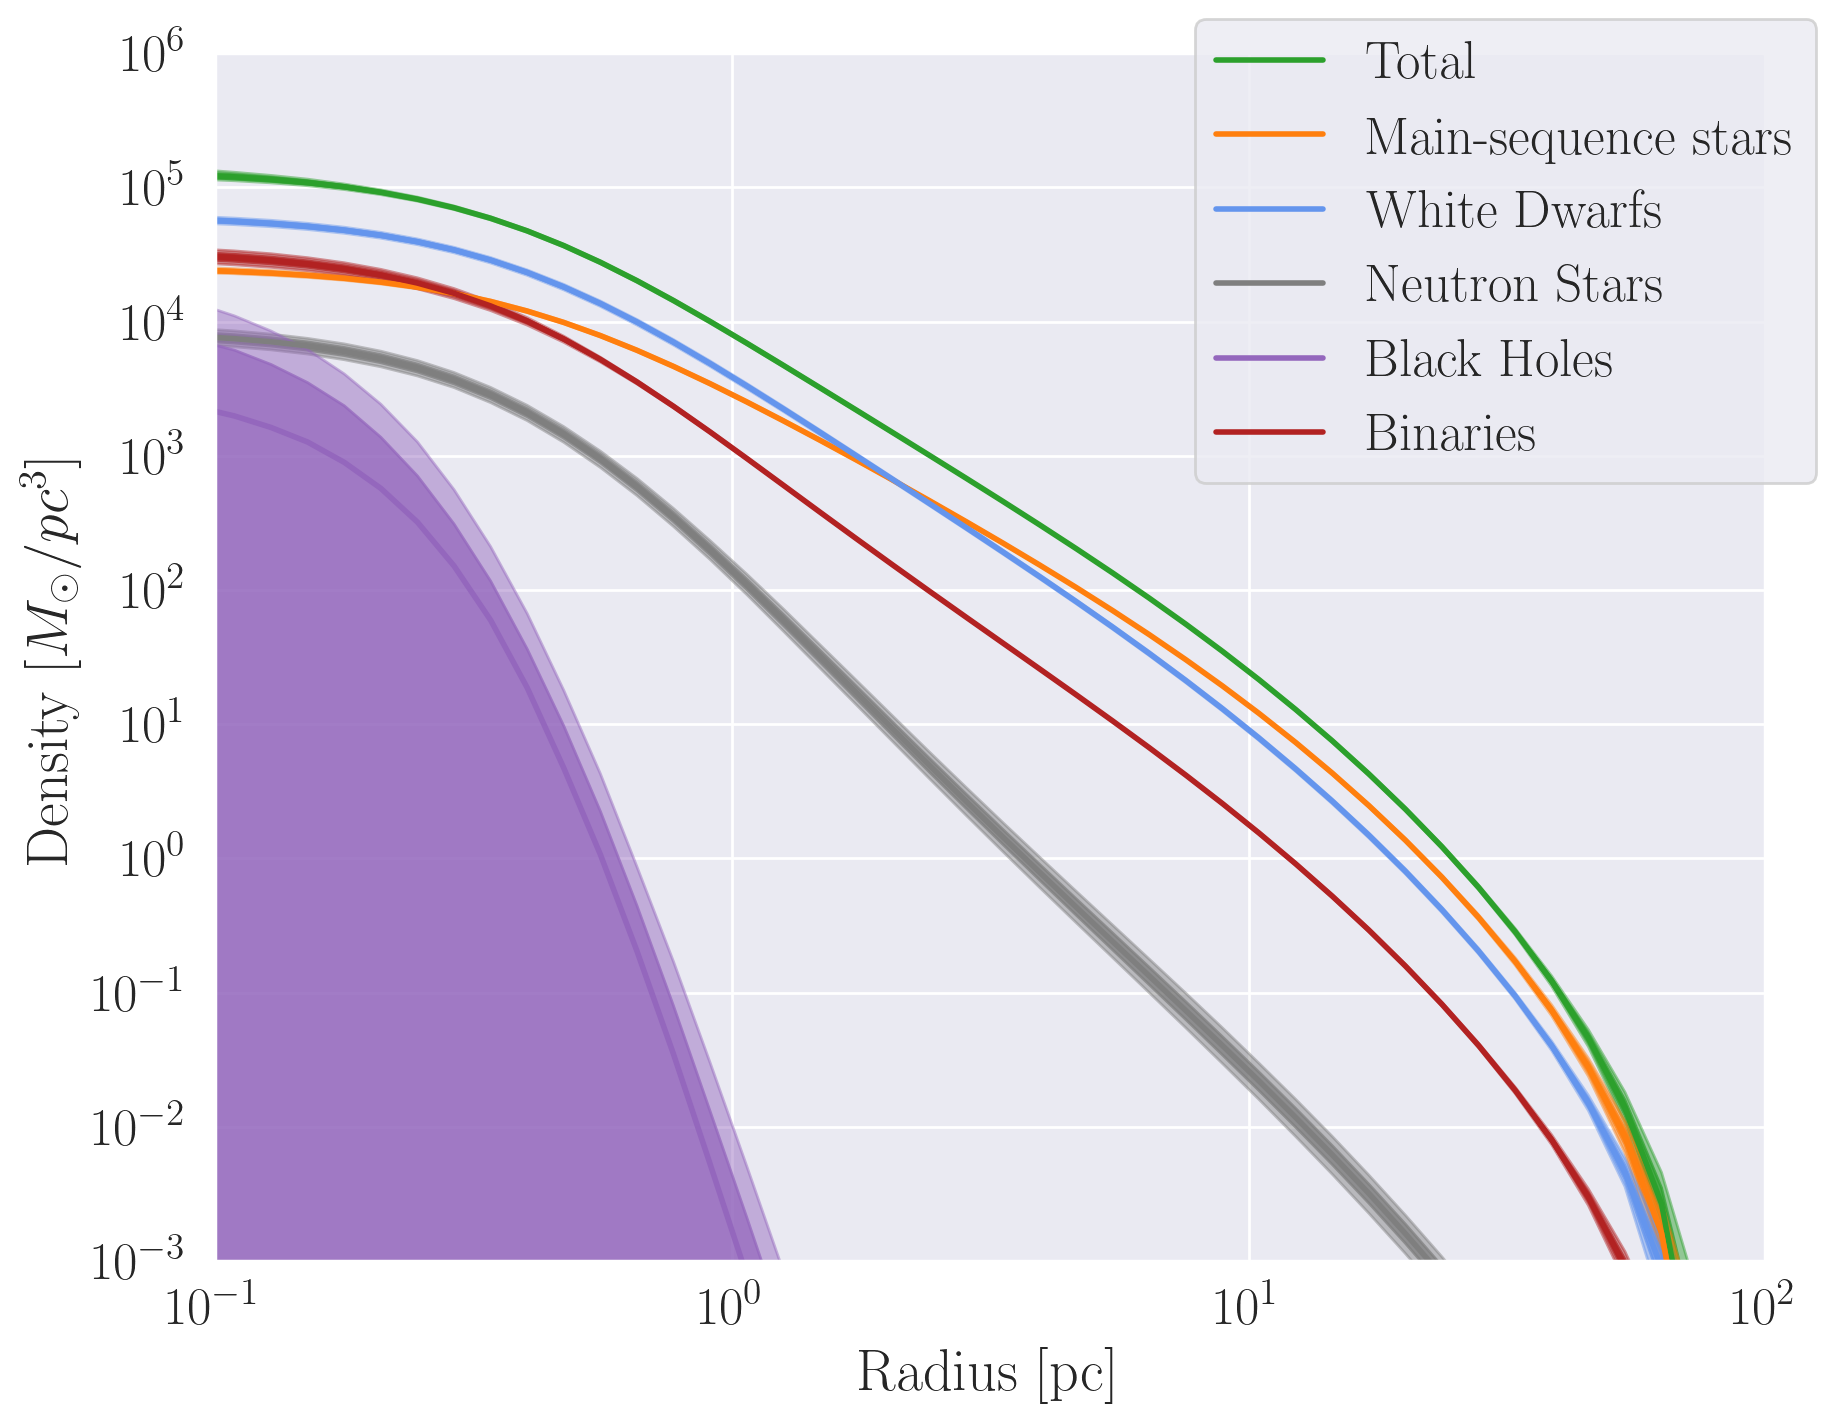
\includegraphics[width=0.8\textwidth]{figures/high_bin_model/density.png}
	\caption{High Binary Densities}
	\label{fig:highbin_model_densities}
\end{figure}



\subsection{Conclusion}

\ps{Implications for past/future work}

\ps{Do binaries in df models actually matter?}








\subsection{Future Work}

We're only looking at binaries in main sequence stars. WD binaries are probably a bigger effect, but
we have no data at all to constrain those quantities, so we ignore them. Maybe looking at N-body or
MC models could give some useful constraints.

Would be nice to look at a cluster where we know there is a larger binary population (NGC3201)and
fit with and without binaries to see what the effects are.